\documentclass[usenames,dvipsnames]{beamer}
\usepackage{../../shared/styles/custom}
\usepackage{../../shared/styles/conventions}

\title{Decision Trees}
\date{\today}
\author{Nipun Batra and teaching staff}
\institute{IIT Gandhinagar}

% Define counter for pop quizzes

\begin{document}
	\maketitle
	
	% Table of Contents
	\begin{frame}
	\frametitle{Table of Contents}
	\tableofcontents
	\end{frame}

\begin{frame}{Information Gain Intuition}
\begin{itemize}
\item For examples, we have 9 Yes, 5 No
	\pause \item Would it be trivial if we had 14 Yes or 14 No?
	\pause \item Yes!
	\pause \item Key insight: Problem is ``easier'' when there is less disagreement
	\pause 	\item Need some statistical measure of ``disagreement'' 
\end{itemize}
\end{frame}

\begin{frame}{Entropy Formula}
$$H(X) = -\sum_{i=1}^k p(x_i) \log_2 p(x_i)$$

\begin{figure}[htp]
    \centering
    \begin{notebookbox}{https://nipunbatra.github.io/ml-teaching/notebooks/entropy.html}
      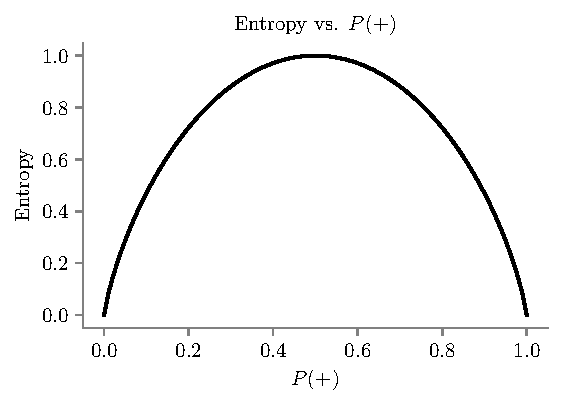
\includegraphics[scale=0.6]{../assets/decision-trees/figures/entropy.pdf}
    \end{notebookbox}
  \end{figure}

\end{frame}
	
\begin{frame}{Root Node Selection}
\begin{itemize}
\item Can we use Outlook as the root node?
				\pause 	\item When Outlook is overcast, we always Play and thus no ``disagreement'' 
\end{itemize}
\end{frame}
	
\begin{frame}{What Does Entropy Measure?}
\textbf{Answer: B) The impurity or ``disagreement'' in a set of examples} - Higher entropy means more mixed classes, lower entropy means more pure subsets.
\end{frame}

\begin{frame}{Entropy Calculation Examples}
\begin{columns}
\begin{column}{.32\textwidth}
	\begin{table}

\begin{tabular}{l|l} \toprule
	\textbf{Outlook} & \textbf{Play} \\ \midrule

	Overcast & Yes  \\
	Overcast & Yes  \\
	Overcast & Yes  \\
	Overcast & Yes  \\ \bottomrule

\end{tabular}
We have 4 Yes, 0 No
$\Entropy = 0$ (pure subset)

	\end{table}

\end{column}

\pause \begin{column}{.32\textwidth}
	\begin{table}
\begin{tabular}{l|l} \toprule
	\textbf{Outlook} & \textbf{Play} \\ \midrule
	Rain     & Yes  \\
	Rain     & Yes  \\
	Rain     & No   \\
	Rain     & Yes  \\
	Rain     & No  \\ \bottomrule
\end{tabular}
We have 3 Yes, 2 No
$\Entropy = -\frac{3}{5} \log_2\left(\frac{3}{5}\right) - \frac{2}{5} \log_2\left(\frac{2}{5}\right) = 0.971$
\end{table}
\end{column}
\end{columns}
\end{frame}

\begin{frame}{Information Gain Calculations}
\begin{itemize}
\item Gain($S_{\text{Outlook=Sunny}}$, Temp) = Entropy(2 Yes, 3 No) - (2/5)*Entropy(0 Yes, 2 No) -(2/5)*Entropy(1 Yes, 1 No) - (1/5)*Entropy(1 Yes, 0 No) 
	\pause \item Gain($S_{\text{Outlook=Sunny}}$, Humidity) = Entropy(2 Yes, 3 No) - (2/5)*Entropy(2 Yes, 0 No) -(3/5)*Entropy(0 Yes, 3 No) $\implies$ \textbf{maximum possible for the set}
	\pause \item Gain($S_{\text{Outlook=Sunny}}$, Windy) = Entropy(2 Yes, 3 No) - (3/5)*Entropy(1 Yes, 2 No) -(2/5)*Entropy(1 Yes, 1 No) 
\end{itemize}
\end{frame}

\begin{frame}{Prediction Example}
Prediction for $<$High Humidity, Strong Wind, Sunny Outlook, Hot Temp$>$ is ? \\
\pause  No
\end{frame}

\begin{frame}{Depth-Limited Trees}
Apply the same rules, except when depth limit is reached, the leaf node is assigned the most common occurring value in that path.

\pause What is depth-$0$ tree (no decision) for the examples? \\
\pause Always predicting Yes

\pause What is depth-$1$ tree (no decision) for the examples? \\
\pause \begin{tikzpicture}[
node/.style={%
	draw,
	rectangle,
},
]

\node [node] (A) {Outlook};
\path (A) ++(-150:\nodeDist) node [node, fill=red] (B) {No};
\path (A) ++(-90:\nodeDist/2) node [node, fill=green] (C) {Yes};
\path (A) ++(-30:\nodeDist) node [node, fill=green] (D) {Yes};

\draw (A) -- (B) node [left,pos=0.25] {Sunny}(A);
\draw (A) -- (C) node [right,pos=0.8] {Overcast}(A);
\draw (A) -- (D) node [right,pos=0.5] {Rain}(A);

\end{tikzpicture}

\end{frame}

\begin{frame}{Why Outlook is Good Root?}
\textbf{Answer: B) When Outlook=Overcast, all examples have Play=Yes} - This creates a pure subset with entropy=0, maximizing information gain.
\end{frame}

\section{Discrete Input, Real Output}

\begin{frame}{Regression Trees}
\begin{itemize}
\item Any guesses?
	\item \pause Mean Squared Error
	\item \pause $\MSE(S) = 311.34$
	\item \pause What about splitting criterion for regression?
	\item \pause \textbf{MSE Reduction} (not Information Gain!)
	\item \pause MSE Reduction = $\MSE(S) - \sum_{v} \frac{|S_v|}{|S|} \MSE(S_v)$
\end{itemize}
\end{frame}

\begin{frame}{Regression Splitting Criterion}
\textbf{Answer: C) Mean Squared Error (MSE) Reduction} - For regression, we minimize MSE instead of maximizing information gain.
\end{frame}

\begin{frame}{Continuous Features}
\textbf{Answer: B) Use midpoints between consecutive sorted feature values} - This ensures we test all meaningful boundaries between different class regions.
\end{frame}

\section{Real Input Real Output}

\begin{frame}{Leaf Node Predictions}
\textbf{Answer: C) The mean of target values in that region} - Each leaf predicts the average target value of training samples that reach that leaf.
\end{frame}

\section{Pruning and Overfitting}

\begin{frame}{The Problem: Overfitting in Decision Trees}
\begin{itemize}
\item \textbf{Unpruned trees}: Can grow very deep and complex
\pause
\item \textbf{Perfect training accuracy}: Each leaf contains single training example
\pause
\item \textbf{But}: Poor generalization to new data
\pause
\item \textbf{Symptoms}:
    \begin{itemize}
    \item High training accuracy, low test accuracy
    \pause
\item Very deep trees with many leaves
    \item Rules that are too specific to training data
    \end{itemize}
\item \textbf{Solution}: Pruning to control model complexity
\end{itemize}
\end{frame}

\begin{frame}{Pre-pruning (Early Stopping)}
\textbf{Stop growing tree before it becomes too complex}:
\begin{itemize}
\item \textbf{Maximum depth}: Limit tree depth (e.g., max\_depth = 5)
\pause
\item \textbf{Minimum samples per split}: Don't split if node has < N samples
\pause
\item \textbf{Minimum samples per leaf}: Ensure each leaf has $\geq$ M samples
\pause
\item \textbf{Maximum features}: Consider only subset of features at each split
\pause
\item \textbf{Minimum impurity decrease}: Only split if improvement > threshold
\end{itemize}

\textbf{Advantages}: Simple, computationally efficient \\
\textbf{Disadvantages}: May stop too early, miss good splits later
\end{frame}

\begin{frame}{Post-pruning (Tree Simplification)}
\textbf{Grow full tree, then remove unnecessary branches}:
\begin{itemize}
\item \textbf{Algorithm}:
    \begin{enumerate}
    \item Grow complete tree on training data
    \pause
\item Use validation set to evaluate subtree performance
    \item Remove branches that don't improve validation accuracy
    \item Repeat until no beneficial removals remain
    \end{enumerate}
\pause
\item \textbf{Cost Complexity Pruning}: Minimize $\text{Error} + \alpha \times \text{Tree Size}$
\pause
\item \textbf{Advantages}: More thorough, can recover from early stopping mistakes
\pause
\item \textbf{Disadvantages}: More computationally expensive
\end{itemize}
\end{frame}

\begin{frame}{Cost Complexity Pruning Algorithm}
\textbf{Systematic approach to find optimal tree size}:
\begin{itemize}
\item \textbf{Cost function}: $R_\alpha(T) = R(T) + \alpha |T|$
    \begin{itemize}
    \item $R(T)$: Misclassification error on validation set
    \pause
\item $|T|$: Number of terminal nodes (tree size)
    \item $\alpha$: Complexity parameter (penalty for larger trees)
    \end{itemize}
\item \textbf{Process}:
    \begin{enumerate}
    \item Start with full tree ($\alpha = 0$)
    \item Gradually increase $\alpha$
    \item At each $\alpha$, prune branches that increase cost
    \item Select $\alpha$ with best cross-validation performance
    \end{enumerate}
\end{itemize}
\end{frame}

\begin{frame}{Bias-Variance Trade-off in Trees}
\begin{itemize}
\item \textbf{Unpruned trees}:
    \begin{itemize}
    \item Low bias (can fit complex patterns)
    \pause
\item High variance (sensitive to training data changes)
    \item Prone to overfitting
    \end{itemize}
\item \textbf{Heavily pruned trees}:
    \begin{itemize}
\item High bias (may miss important patterns)
    \item Low variance (more stable predictions)
    \pause
\item Risk of underfitting
    \end{itemize}
\item \textbf{Optimal pruning}: Balances bias and variance
\item \textbf{Cross-validation}: Essential for finding this balance
\end{itemize}
\end{frame}

\begin{frame}{Practical Pruning Guidelines}
\begin{itemize}
\item \textbf{Start simple}: Begin with restrictive pre-pruning parameters
\pause
\item \textbf{Cross-validation}: Always use CV to select pruning parameters
\pause
\item \textbf{Validation curves}: Plot training/validation error vs. tree complexity
\pause
\item \textbf{Common parameters} (sklearn):
    \begin{itemize}
    \item \texttt{max\_depth}: Start with 3-10
    \pause
\item \texttt{min\_samples\_split}: Try 10-100
    \item \texttt{min\_samples\_leaf}: Try 5-50
    \item \texttt{ccp\_alpha}: Use for cost complexity pruning
    \end{itemize}
\item \textbf{Domain knowledge}: Consider interpretability requirements
\end{itemize}
\end{frame}

\section{Summary and Key Takeaways}

\begin{frame}{Summary}
\begin{itemize}
\item Interpretability an important goal
\item Decision trees: well known interpretable models
\pause
\item Learning optimal tree is hard
\item Greedy approach:
\item Recursively split to maximize “performance gain”
\pause
\item Issues:
\begin{itemize}
	\item Can overfit easily!
	\item Empirically not as powerful as other methods
\end{itemize}
\end{itemize}

\end{frame}

\begin{frame}

	\begin{figure}
		\centering
		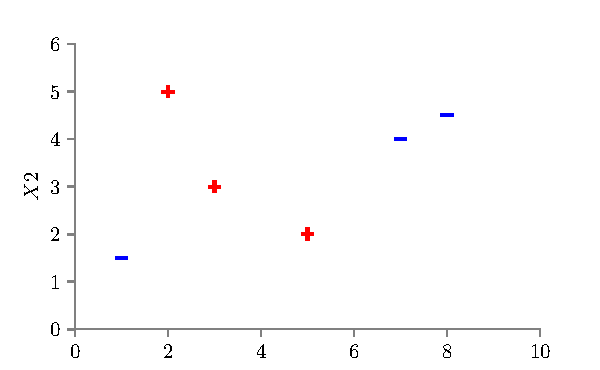
\includegraphics{../assets/decision-trees/figures/dt_weighted/fig1.pdf}
	\end{figure}

	\end{frame}

	\begin{frame}
	
	\begin{figure}
		\centering
		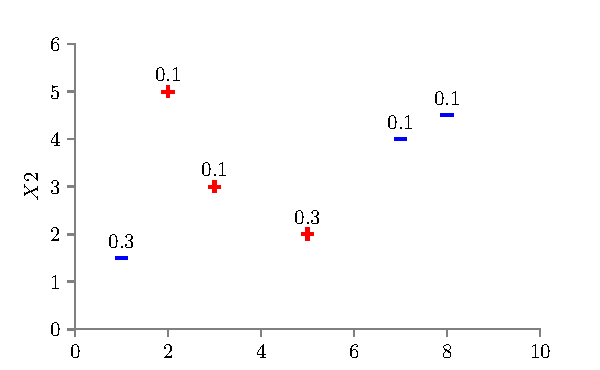
\includegraphics{../assets/decision-trees/figures/dt_weighted/fig2.pdf}
	\end{figure}

	\end{frame}

	\begin{frame}
	
	\begin{figure}
		\centering
		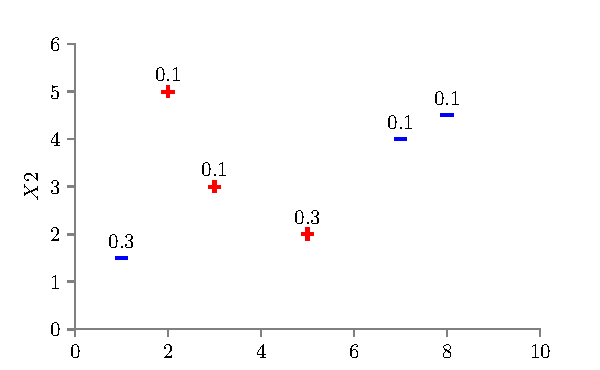
\includegraphics{../assets/decision-trees/figures/dt_weighted/fig2.pdf}
	\end{figure}
	
	$$\Entropy = -P(+) \log_2 P(+) - P(-) \log_2 P(-)$$
	
	$$P(+) = \frac{0.1 + 0.1 + 0.3}{1} = 0.5, \quad P(-) = \frac{0.3 + 0.1 + 0.1}{1} = 0.5$$
	
	$$\Entropy = E_s = -\frac{1}{2} \log_2 \frac{1}{2} - \frac{1}{2} \log_2 \frac{1}{2} = 1$$
	
	\end{frame}

	\section{Weighted Entropy}

	\begin{frame}
	
	\begin{figure}
		\centering
		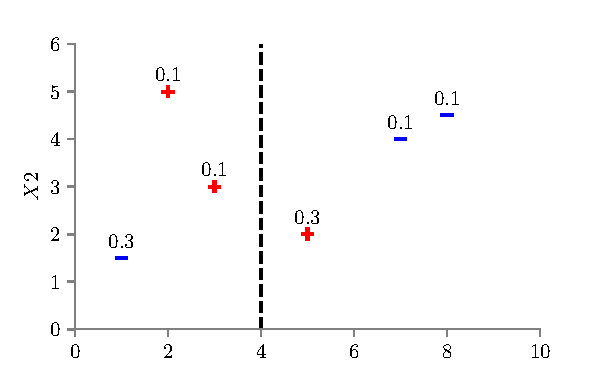
\includegraphics{../assets/decision-trees/figures/dt_weighted/fig3.pdf}
	\end{figure}

	Candidate Line: \(X1 = 4 (X1^*)\)

	\end{frame}

	\begin{frame}
	\begin{figure}
		\centering
		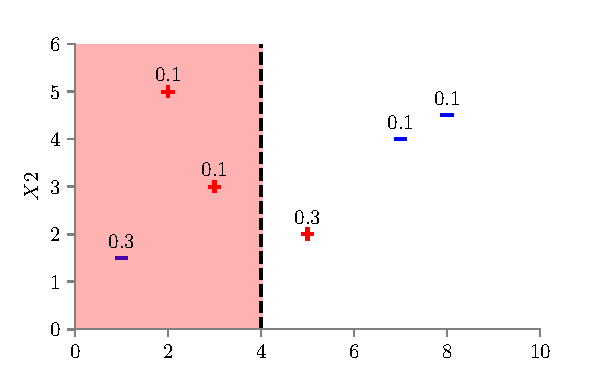
\includegraphics{../assets/decision-trees/figures/dt_weighted/fig4.pdf}
	\end{figure}
	
	Entropy of \(X1 \leq X1^*  = E_{S(X1 < X1^*)}\)
	
	$$P(+) = \frac{0.1 + 0.1}{0.1 + 0.1 + 0.3} = \frac{2}{5}$$
	
	$$P(-) = \frac{3}{5}$$

	\end{frame}

	\begin{frame}
	
	\begin{figure}
		\centering
		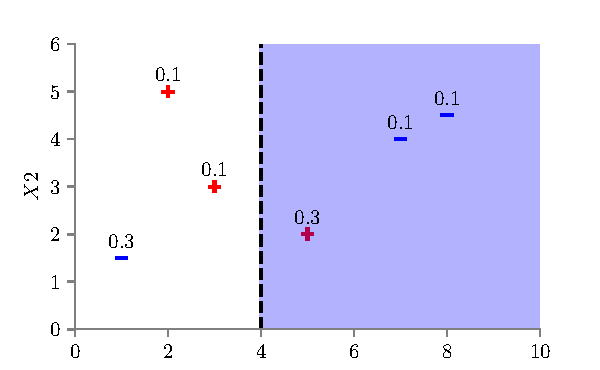
\includegraphics{../assets/decision-trees/figures/dt_weighted/fig5.pdf}
	\end{figure}
	Entropy of $X_1 > X_1^* = E_{S(X_1 > X_1^*)}$
	
	$$P(+) = \frac{3}{5}$$
	
	$$P(-) = \frac{2}{5}$$
	
	\end{frame}

	\begin{frame}
	
	\begin{figure}
		\centering
		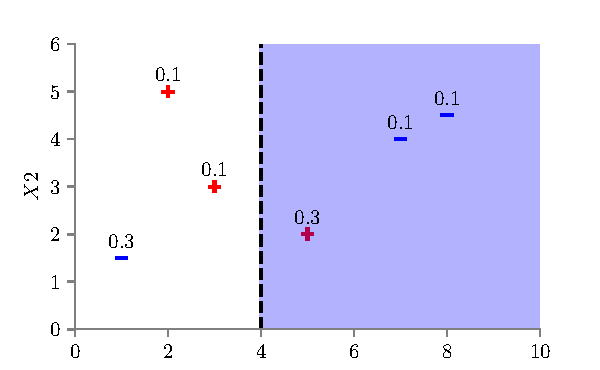
\includegraphics{../assets/decision-trees/figures/dt_weighted/fig5.pdf}
	\end{figure}
	
	$$\text{IG}(X_1 = X_1^*) = E_S - \frac{0.5}{1} \cdot E_{S(X_1 < X_1^*)} - \frac{0.5}{1} \cdot E_{S(X_1 > X_1^*)}$$
	
	\end{frame}

\end{section}
\end{document}
